\section{Algorithmic construction}
\label{sec:main-algorithm}

% Please keep main-text Step targets local and the shared appendix names intact.
\newcommand{\MainAlgoBlockTarget}[1]{%
  \hypertarget{main-algo-block-#1}{\AlgoBlockHeading{#1}}}
\newcommand{\MainAlgoInlineTarget}[1]{%
  \hypertarget{main-algo-block-#1}{%
    \textbf{\AlgoStepPrefix~\AlgoBlockCode{#1}. \AlgoBlockName{#1}.}}}
\newcommand{\MainAlgoShortTarget}[1]{%
  \hypertarget{main-algo-block-#1}{\textbf{\AlgoStepPrefix~\AlgoBlockCode{#1}.}}}
\DeclareRobustCommand{\MainAlgoBlockRef}[1]{%
  \hyperlink{main-algo-block-#1}{\AlgoStepPrefix~\AlgoBlockCode{#1}}}

% This bounded Section 4 rewrite is red for author review; the figure keeps
% semantic colors. The formal low-degree lemma now lives in the appendix.
{\color{red}
We now construct the sampler in \cref{main:thm:upper-curve}.
The key is to learn the residual forest as sampling removes vertices.
\MainAlgoBlockRef{draft}--\MainAlgoBlockRef{screen} share counterfactual
probes to recover low-degree neighborhoods with high probability.
When all screens succeed, \MainAlgoBlockRef{peel} uses these reports to
shrink the high-degree core by singleton commits, and
\MainAlgoBlockRef{terminal}--\MainAlgoBlockRef{centroid} recover the
remaining forest for parallel centroid commits
(Algorithm~\ref{main:alg:upper-bound-sampler}).

\begin{algorithm}[H]
\caption{\textcolor{red}{Counterfactual-probing sampler: shared tests, claim-based peeling, and centroid commits. Full safeguards: \cref{app:alg:complete-sampler}.}}
\label{main:alg:upper-bound-sampler}
{\color{red}\small
% Please use repeat with an explicit break, while retaining normal indentation.
\algrenewtext{Loop}{\textbf{repeat}}
\algtext*{EndLoop}
\algtext*{EndFor}
\begin{algorithmic}[1]
\Statex \textbf{Input:} $N$, ordered vocabulary $\Vocab$, frozen oracle $\FrozenOracle$, accuracy $\TargetTolerance$
\Statex \textbf{Parameters:} $\DegreeCutoff,\ChunkCount,\ThresholdFloor,\TailTolerance,p,\RandomColoringCount$
  (\cref{app:cor:fixed-accuracy-main})
\State \MainAlgoInlineTarget{preprocess}
\Loop
  \State \MainAlgoInlineTarget{draft} Fix a draft; draw fresh independent colorings
  \State \MainAlgoInlineTarget{screen}
  \For{each coloring $\tau=1,\ldots,\RandomColoringCount$}
    \State \MainAlgoShortTarget{chunks} Split each readout color class into chunks
    \For{each nonempty chunk $\mathcal C$ and other source color}
      \For{each bank-or-tail column $\kappa$}
        \State \MainAlgoShortTarget{probes} Submit the packed state; retain replies at $j\in\mathcal C$
      \EndFor
    \EndFor
  \EndFor
  \State \MainAlgoShortTarget{aggregate} Compute votes, strict majorities, and capped rows $\ScreenRow{j}$
  \State \MainAlgoInlineTarget{peel} Form $\PeelSet$; if empty or at the phase cap, \textbf{break}
  \State Freeze $\PeelSet$ and commit its vertices singly in public order
\EndLoop
\State \MainAlgoInlineTarget{terminal}\enspace \MainAlgoInlineTarget{centroid}
\end{algorithmic}
}
\end{algorithm}

% Please include the author-supplied PDF unchanged and retain the existing label.
% Source attachment: de757cd7-77d6-4058-9436-f652c5046293/fig2_votes.pdf.
% SHA-256: a3f79400cdf48f23196f4c553b87d2c0fa6c1faa968b9c86b879c59ebb532041.
% The previous TikZ version remains available but is not compiled here.
\begin{figure}[H]
\centering
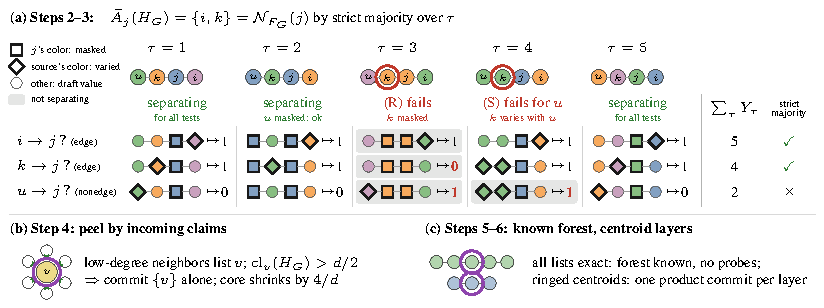
\includegraphics[width=\linewidth]{figures/algorithm_examples_2026-09-18/fig2_votes_2026-09-26_002617_JST.pdf}
\caption{\textcolor{red}{Shared tests and majority recovery.
(a) Each cell represents all bank/tail columns; each readout color has one
chunk. Equal-color pairs (no diamond) get vote $0$ without probing.
Grey: nonseparation; red: illustrative errors.
(b) Singleton peels contract the core per phase.
(c) One centroid per component forms a terminal batch.}}
\label{fig:algorithm-overview-20260918}
\end{figure}


\subsection{Building a single-source edge test}
\label{sec:main-algorithm-flow}

We prepare the edge test that \cref{sec:main-packed-screen} will share across pairs.
Fix a history $\History=(G,x_G)$, distinct residual positions $i,j$, and
a query-free draft $\DraftFiller$.
The single-source state $y^a$ reveals $x_G$, sets
$y_i^a=a$, masks $j$, and fixes all other residual coordinates to their draft
values (Figure~\ref{fig:intro-counterfactual-20260920}).
Its exact reply $\BoundaryRow{i}{j}{a}{z}$ has boundary
$z=(x_G,\DraftFiller_{\ResidualPositions\setminus\{i,j\}})$.
For a nonedge this row is constant in $a$ by forest separation
(\cref{app:lem:residual-markov});
for an edge its TV diameter is at least $\EdgeSignal$ by
\cref{main:ass:uen} (UEN).
Testing all ordered pairs and tokens separately costs
$|\ResidualPositions|(|\ResidualPositions|-1)\VocabSize$ submissions.

\textbf{Banks and tail representatives (\MainAlgoBlockRef{preprocess}).}
To reduce token choices, we test a local vocabulary bank and one
representative of the omitted tokens.
Write $\RowTVError:=\TargetTolerance/(2\sqrt N)$ for the row-TV error
bound in either case (\cref{app:eq:oracle-tv-radius,app:eq:kl-oracle-inclusion}).
On the threshold grid $\ThresholdGrid$ with floor $\ThresholdFloor$,
choose $\TailThreshold=\max\{u\in\ThresholdGrid:u\le\TailTolerance\}$,
the largest threshold allowed by the tail budget.
One all-mask submission gives the local vocabulary banks
$\TokenBank{i}:=\{a\in\Vocab:\OracleRowMass{\MASK^N}{i}{a}
\ge\TailThreshold-\RowTVError\}$ and tail representatives
$\TailRepresentative{i}=\min_{\TokenOrder}(\Vocab\setminus\TokenBank{i})$
(\cref{app:def:preprocessing}).
The standard draft reuses these rows without another submission
(\cref{app:eq:standard-draft}).

\cref{main:ass:rt} (RT) allows each omitted token to be replaced by $\TailRepresentative{i}$
within TV error $\TailTolerance=\EdgeSignal/2$.
\cref{main:ass:frequency-envelope} (RF) bounds
$\MaxBankSize=\max_i|\TokenBank{i}|=O(\EdgeSignal^{-1/\RankTailExponent})$.

\textbf{A resolvable edge signal.}
The test queries every bank token and the tail representative, then compares
$\max_{a,a'\in\TokenBank{i}\cup\{\TailRepresentative{i}\}}
\dTV(\OracleRow{y^a}{j},\OracleRow{y^{a'}}{j})$ with $2\RowTVError$.
This observed diameter is at most $2\RowTVError$ for a nonedge;
for an edge it is at least
$\EdgeSignal-\TailTolerance-2\RowTVError>2\RowTVError$
when $\ScreenResolution:=4\RowTVError+\TailTolerance<\EdgeSignal$.
Under the scaling in \cref{main:ass:main-scaling}, our parameter choices
make preprocessing feasible and ensure $\ScreenResolution<\EdgeSignal$
for all sufficiently large $N$ (\cref{app:cor:fixed-accuracy-main}).
\AppLowDegreeScreenRef\ proves the diameter bound.

\subsection{Packing tests with random colorings}
\label{sec:main-packed-screen}

We share the tests of \cref{sec:main-algorithm-flow} across source and readout groups.
For each coloring, \MainAlgoBlockRef{chunks} splits color classes into
chunks of at most $\lceil N/\ChunkCount\rceil$ positions.
\MainAlgoBlockRef{probes} masks one chunk and varies another color class
through bank-or-tail columns $\kappa$: each source takes its own token value,
while committed values and the remaining draft stay fixed.
There are $\ScreenColumnCount\le\MaxBankSize+1$ submitted columns;
\cref{app:eq:packed-column,app:eq:screen-column-count} specify padding
and the empty-bank case.
The same replies test every source--readout pair between the two groups.
\MainAlgoBlockRef{draft} draws $\RandomColoringCount$ independent colorings
with independent uniform colors $\ColorHash{\tau}{i}\in[p]$, $p=8(\DegreeCutoff+1)$.
All screen probes are fixed before replies: one oracle stage
(\cref{app:alg:packed-screen}).
Coloring also shares evaluations in sparse Jacobian
estimation~\citep{coleman1983estimation}.

For $i\to j$, the single-source test is preserved if every neighbor of $j$
is revealed and all except $i$ stay fixed. Call a coloring \emph{separating} when:
\begingroup
% Please keep the list indentation local and retain the standard vertical spacing.
\setlength{\leftmargini}{2pc}
\begin{itemize}
\item \emph{Readout separation (R).} No neighbor of $j$ has $j$'s color,
so none is masked.
\item \emph{Source separation (S).} No neighbor of $j$ other than $i$ has
$i$'s color, so none varies with $i$.
\end{itemize}
\endgroup
For separating colorings with distinct source/readout colors, exact replies
equal their single-source counterparts (\cref{app:lem:fixed-draft-rows}).
Figure~\ref{fig:algorithm-overview-20260918}(a) shows possible collision errors
and majority voting.

\textbf{Voting and capped candidate lists (\MainAlgoBlockRef{aggregate}).}
Each coloring casts one vote on whether $i$ and $j$ are adjacent, using
the shared replies from \MainAlgoBlockRef{probes}.
For differently colored $i,j$, compare the conditional distributions
returned at $j$ across the columns probing $i$'s color class.
Let $\ScreenDiameter{\tau}{i}{j}$ be their maximum pairwise TV distance
(\cref{app:eq:observed-screen-diameter}).
Applying the threshold from \cref{sec:main-algorithm-flow} gives the vote
$\ScreenVote{\tau}{i}{j}
=\mathbf1\{\ScreenDiameter{\tau}{i}{j}>2\RowTVError\}$.
Equal-color pairs have no corresponding probe and receive vote zero.
We retain candidates supported by a strict majority of all
$\RandomColoringCount$ colorings:
\[
\CandidateRow{j}:=\left\{i\in\ResidualPositions\setminus\{j\}:
\sum_{\tau=1}^{\RandomColoringCount}\ScreenVote{\tau}{i}{j}>
\RandomColoringCount/2\right\}.
\]
The returned list $\ScreenRow{j}$ equals $\CandidateRow{j}$ when it contains
at most $\DegreeCutoff$ candidates; otherwise, it retains the $\DegreeCutoff$
candidates with the highest vote totals, breaking ties by public position order.
Random hashing followed by majority aggregation also appears in junta
learning~\citep{bshouty2018exact}.

\textbf{Low-degree recovery (\MainAlgoBlockRef{draft}--\MainAlgoBlockRef{screen}).}
For a readout $j$ with $d_{\ResidualForest}(j)\le\DegreeCutoff$,
conditions (R) and (S) forbid at most $2\DegreeCutoff$ color equalities.
Conditional on the past and the fixed draft, each equality has probability
$1/p$. Thus, each fresh coloring separates any fixed pair $(i,j)$ with
probability at least $1-2\DegreeCutoff/p>3/4$.

By the single-source margin $\ScreenResolution<\EdgeSignal$ from
\cref{sec:main-algorithm-flow}, every separating coloring gives the correct
edge/nonedge vote.
This includes same-color separating pairs: condition (R) excludes an edge,
so their zero vote is correct.
A strict separating majority therefore classifies the pair correctly,
regardless of the remaining votes.
Let $\ScreenSuccess{\History}$ denote the analysis-only event that such a
majority holds for every $i\ne j$ with
$d_{\ResidualForest}(j)\le\DegreeCutoff$.
On this event, each low-degree candidate list equals the true neighborhood.
Its size is already at most $\DegreeCutoff$, so truncation leaves it
unchanged (\cref{app:lem:low-degree-screen}):
\begin{equation}
 \ScreenRow{j}=\mathcal N_{\ResidualForest}(j)
 \quad\text{for every }j\in\ResidualPositions
 \text{ with }d_{\ResidualForest}(j)\le\DegreeCutoff.
 \label{main:eq:exact-low-degree-row}
\end{equation}

By independence across colorings, Hoeffding's inequality bounds the
probability that a fixed pair lacks a strict separating majority by
$e^{-\RandomColoringCount/8}$. A union bound over pairs gives
\begin{equation}
 \Pr\bigl(\ScreenSuccess{\History}^{\mathsf c}
       \mid\text{past including the current draft}\bigr)
 \le N^2e^{-\RandomColoringCount/8}.
 \label{main:eq:conditional-screen-success}
\end{equation}
Fresh colors make this bound valid at every adaptively reached screen.
A further union bound over the capped number of screen calls controls
failure along the full execution (\cref{app:lem:random-screen-success}).

\subsection{Peeling the high-degree core, then centroid layers}
\label{sec:main-peeling-terminal}

\MainAlgoBlockRef{peel} commits vertices with many incoming neighbor reports singly.
When all screens succeed, repeated peeling removes the high-degree core,
enabling forest recovery and parallel centroid commits
(\MainAlgoBlockRef{terminal}--\MainAlgoBlockRef{centroid}).

Define the incoming claim count and the peel set
(also \cref{app:eq:claim-and-peel-set}) by
\begin{equation}
 \ClaimCount{v}
 :=|\{u\in\ResidualPositions:v\in\ScreenRow{u}\}|,
 \qquad
 \PeelSet:=\{v\in\ResidualPositions:\ClaimCount{v}>\DegreeCutoff/2\}.
 \label{main:eq:claim-and-peel-set}
\end{equation}

\textbf{Why peel by incoming claims (\MainAlgoBlockRef{peel})?}
A high-degree vertex's own report may be unreliable, but each low-degree
neighbor reports it correctly.
Peeling may also select low-degree vertices; singleton
commits introduce no within-batch dependence error.
The size cap controls their cost: on successful screens,
$|\ScreenRow{u}|\le d_{\ResidualForest}(u)$, so
\[
 (\DegreeCutoff/2)|\PeelSet|
 \le\sum_v\ClaimCount{v}
 =\sum_u|\ScreenRow{u}|
 \le\sum_u d_{\ResidualForest}(u)<2|\ResidualPositions|.
\]
Thus a phase uses fewer than $4|\ResidualPositions|/\DegreeCutoff$
singleton rounds.

\textbf{The high-degree core shrinks.}
Let $\HighDegreeSet=\{v:d_{\ResidualForest}(v)>\DegreeCutoff\}$.
On a successful screen, an unpeeled high-degree vertex has at most $\DegreeCutoff/2$ low-degree
neighbors, since each contributes a claim; it therefore has more than
$\DegreeCutoff/2$ neighbors in $\HighDegreeSet$.
The forest induced on $\HighDegreeSet$ has degree sum below
$2|\HighDegreeSet|$, so fewer than
$(4/\DegreeCutoff)|\HighDegreeSet|$ high-degree vertices remain unpeeled
when $\HighDegreeSet$ is nonempty.
Deleting vertices cannot raise degrees; the next history $\History'$ satisfies
\begin{equation}
 |\HighDegreeSetAt{\History'}|
 \le(4/\DegreeCutoff)|\HighDegreeSet|.
 \label{main:eq:peeling-contraction}
\end{equation}

\textbf{Finish without further probes (\MainAlgoBlockRef{terminal}--\MainAlgoBlockRef{centroid}).}
On successful-screen paths, the $O(\log N)$ phase cap or an empty peel set
ensures residual maximum degree at most $\DegreeCutoff$
(\cref{app:lem:successful-path-structure}).
Since screening precedes either test,
\cref{main:eq:exact-low-degree-row} makes every terminal row exact.
Joining reported neighbors therefore recovers the true residual forest.
The exact joint conditional of one centroid per component factorizes.
Centroid deletion halves component sizes, giving logarithmically many layers
(\cref{app:lem:residual-markov,app:lem:forest-basics}).
These layers form a vertex ranking~\citep{iyer1988optimal}, with higher ranks
assigned to earlier commits.
Only commit submissions remain: later steps delete vertices of the known
forest rather than rediscovering it.

\subsection{Resources and accuracy}
\label{sec:main-algorithm-resources}

Each screen uses at most
$\ScreenColumnCount\RandomColoringCount p(p+\ChunkCount)$ submissions:
columns, colorings, source colors, and readout chunks.
With $\ChunkCount=\DegreeCutoff$, the bank bound, phase count, and peel-size
bound yield
\[
 \CounterfactualQueries
 =\widetilde O(\EdgeSignal^{-1/\RankTailExponent}\DegreeCutoff^2),
 \qquad
 \CommitRounds,\OracleDepth=\widetilde O(N/\DegreeCutoff).
\]
Larger $\DegreeCutoff$ increases screening cost but reduces commit rounds;
balancing gives
\cref{main:eq:balanced-upper}.
Public caps enforce the bounds even on failed-screen paths
(\cref{app:lem:upper-resources}); \cref{app:alg:complete-sampler} specifies
singleton cycle repair and the round-cap all-residual product-commit fallback.

On paths where all screens succeed, the target conditional factorizes over
every commit batch.
The appendix bounds oracle error and the contribution of failed screens
using separate TV and forward-KL arguments
(\cref{app:lem:exact-hybrid,app:lem:adaptive-hellinger-upper,app:lem:safe-controller-comparison,app:thm:finite-kl-upper}).
The calibration in \cref{app:cor:fixed-accuracy-main} gives the guarantees
of \cref{main:thm:upper-curve} for the sampler in
Algorithm~\ref{main:alg:upper-bound-sampler}.
}
